\documentclass[runningheads,a4paper]{llncs}

%
\usepackage{amssymb}
\usepackage{amsmath}
\usepackage{url}
\usepackage{graphicx}
\usepackage{multirow}
%
\newcommand{\argmin}[1]{\underset{#1}{\operatorname{arg}\operatorname{min}}\;}
\mathchardef\mhyphen="2D
\raggedbottom 
%
% Allow easy processing of labeled images in figures
\newcounter{lfigcounter}
\newenvironment{IonTab}{\begin{table}[htb]}{\end{table}}
\newenvironment{IonFig}{\setcounter{lfigcounter}{1}\begin{figure}} {\end{figure}}
\newenvironment{IonFigH}{\setcounter{lfigcounter}{1}\begin{figure}[h]}{\end{figure}}
\newenvironment{IonFigT}{\setcounter{lfigcounter}{1}\begin{figure}[!t]}{\end{figure}}
\newenvironment{IonFigB}{\setcounter{lfigcounter}{1}\begin{figure}[b]}{\end{figure}}
\def\ionbox#1{\makebox[#1]{(\alph{lfigcounter})}\stepcounter{lfigcounter}}
%
\begin{document}

\mainmatter  % start of an individual contribution

% first the title is needed
\title{An Image-based method for phase estimation, gating and temporal super-resolution of \\cardiac ultrasound}

% a short form should be given in case it is too long for the running head
\titlerunning{Image-based Phase Estimation Method for Cardiac Ultrasound}

% the name(s) of the author(s) follow(s) next
%
% NB: Chinese authors should write their first names(s) in front of
% their surnames. This ensures that the names appear correctly in
% the running heads and the author index.
%

% anonymous stuff
\author{*}
\authorrunning{*}   
\tocauthor{*}
\institute{*}

\maketitle

\begin{abstract}
Point-of-care low-cost hand-held ultrasound devices are emerging as an increasingly effective tool for rapid non-invasive visual assessment of cardiac structure and function on the bed-side. Their diagnostic value can be enriched further by coupling them with automated image analysis algorithms to accurately detect and quantify any cardiac abnormalities at the point-of-care potentially even in asymptomatic patients. However, a major challenge to this is the poor spatio-temporal resolution and high noise level of images obtained using these devices. In an effort to address this problem, we present a novel method for de-noising, gating, and temporal super-resolution of noisy low frame-rate periodic image sequences such as the ones obtained using low-cost hand-held cardiac ultrasound devices. We first leverage the inherent image-level redundancy in a periodic image sequence to decouple signal from noise using a low-rank + sparse decomposition algorithm. Next, we transform the complex high-dimensional periodic image sequence to a narrow-band 1D time series with the same periodicity characteristics using a novel strategy based on inter-frame similarity. Next, we decompose this time series use a season-trend decomposition method to obtain the heart-beat (season) and respiratory (trend) signals. Next, we use the Hilbert transform to estimate the instantaneous cardiac and respiratory phases of each frame to facilitate gating and super-resolution. Lastly, we use Nadarya-Watson kernel regression to construct an image manifold parameterized by intra-period phase which can then be sampled to reconstruct a de-noised single-period image sequence at a higher temporal-resolution. We demonstrate the utility and efficacy of our method both on synthetic data and on real image sequences of the beating heart acquired using a low-cost hand-held ultrasound device.
%\keywords{Cardiac, Ultrasound, Phase estimation, Gating, Temporal super-resolution}
\end{abstract}

\vspace{-0.5cm}
\section{Introduction}
\label{sec:intro}
%

%

%\vspace{-0.5cm}
\section{Method}
\label{sec:method}
%
In this section, we present the theory underlying the proposed methods for instantaneous phase estimation, gating and temporal super-resolution of cardiac ultrasound videos. Specifically, we begin by describing our method for the estimation of instantaneous cardiac and respiratory phases in Section \ref{sec:method:phase_estimation}. We then present a robust method that uses these phase estimates to gate out video frames predominantly influenced by respiratory motion in Section \ref{sec:method:gating}. Finally, in Section \ref{sec:method:super_resolution}, we present a kernel regression method that uses the phase-tagged image sequence to reconstruct a single-period video at higher-temporal resolution. 
%
%
\begin{IonFigT}
\centering
%
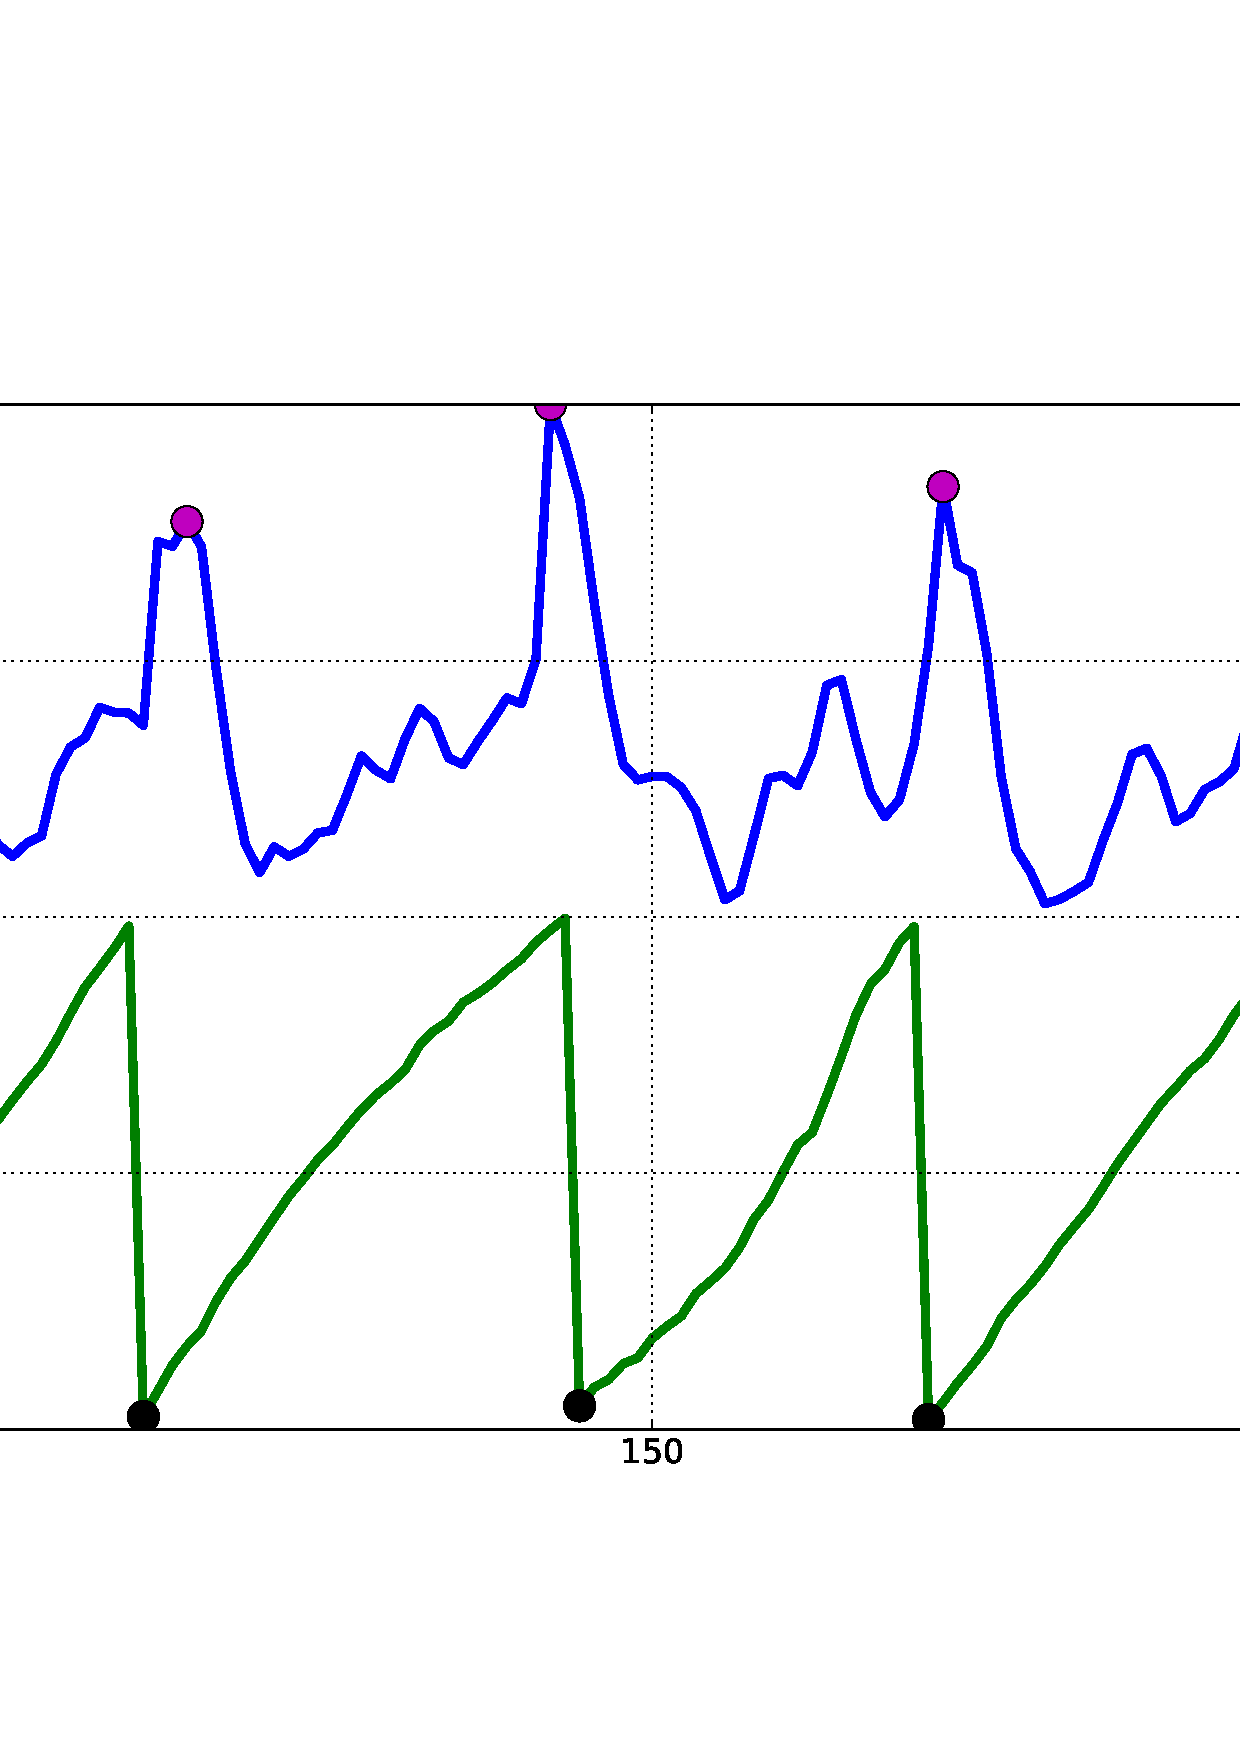
\includegraphics[width=5.0in]{figures/decoded/2015-07-27-10-36-06_2015-07-15-16-56-16_1.raw.bmode/ecg_instaphase_overlay.png}\\
\ionbox{5.0in}\\
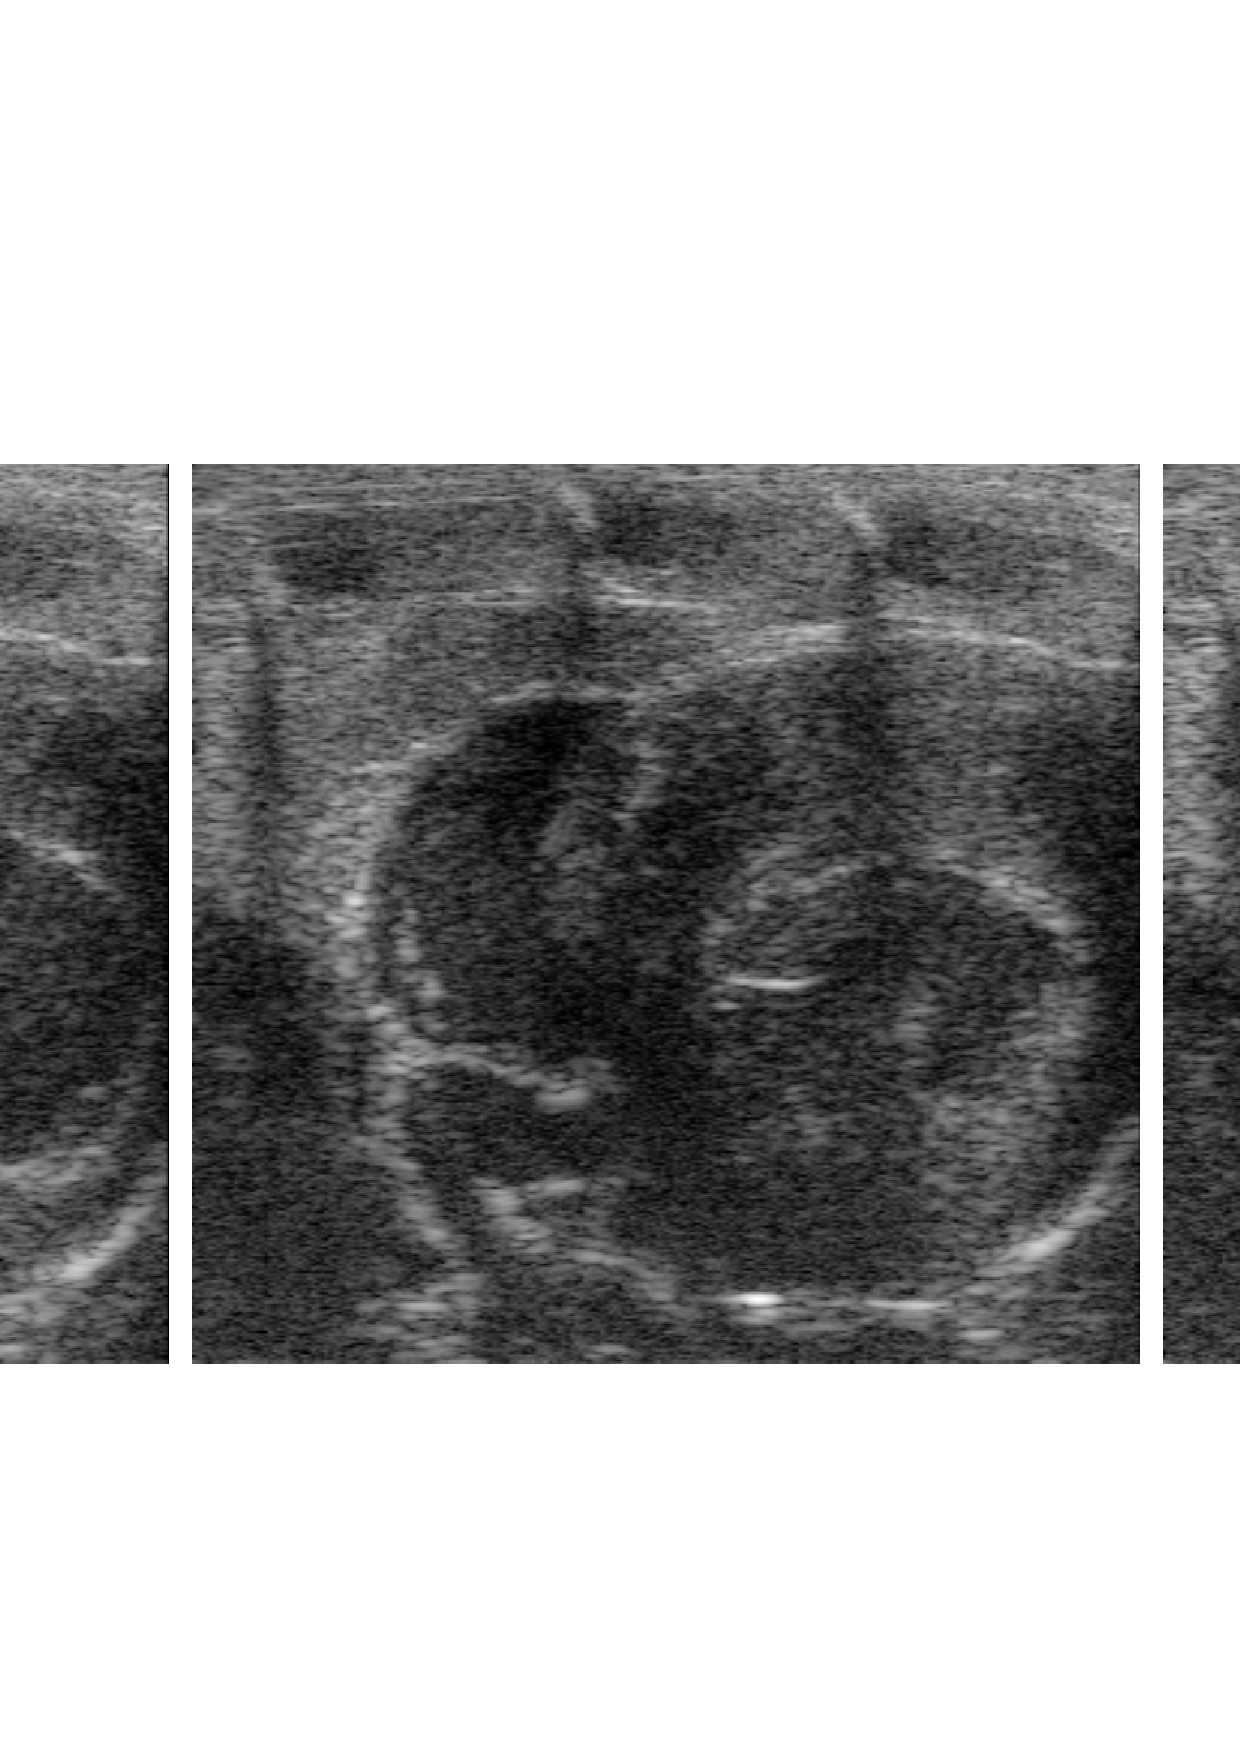
\includegraphics[width=5.0in]{figures/decoded/2015-07-27-10-36-06_2015-07-15-16-56-16_1.raw.bmode/qrs_peak_to_peak.png}
\ionbox{5.0in}\\
\includegraphics[width=5.0in]{figures/decoded/2015-07-27-10-36-06_2015-07-15-16-56-16_1.raw.bmode/instaphase_valley_to_valley.png}
\ionbox{5.0in}\\
%
\caption{Illustration of correspondence between ECG and the instantaneous cardiac phase estimated using the proposed method: (a) ECG signal (blue) and the cardiac phase estimated using our method using only image data. Also shown are the peaks of the QRS complex (pink circle) and the minima of the estimated cardiac phase (black circle) that correspond to the QRS peaks, (b) Five video frames evenly spaced in time between the first and second QRS peaks of the ECG signal constituting one cardiac cycle, and (c) Five video frames evenly spaced in time between first and second minima of the estimated cardiac phase constituting one cardiac cycle.}
\label{fig:instaphase_vs_ecg}
\end{IonFigT}
%\vspace{-0.5cm}
\subsection{Estimation of instantaneous cardiac and respiratory phases}
\label{sec:method:phase_estimation}
%
\begin{IonFigT}
\centering
%
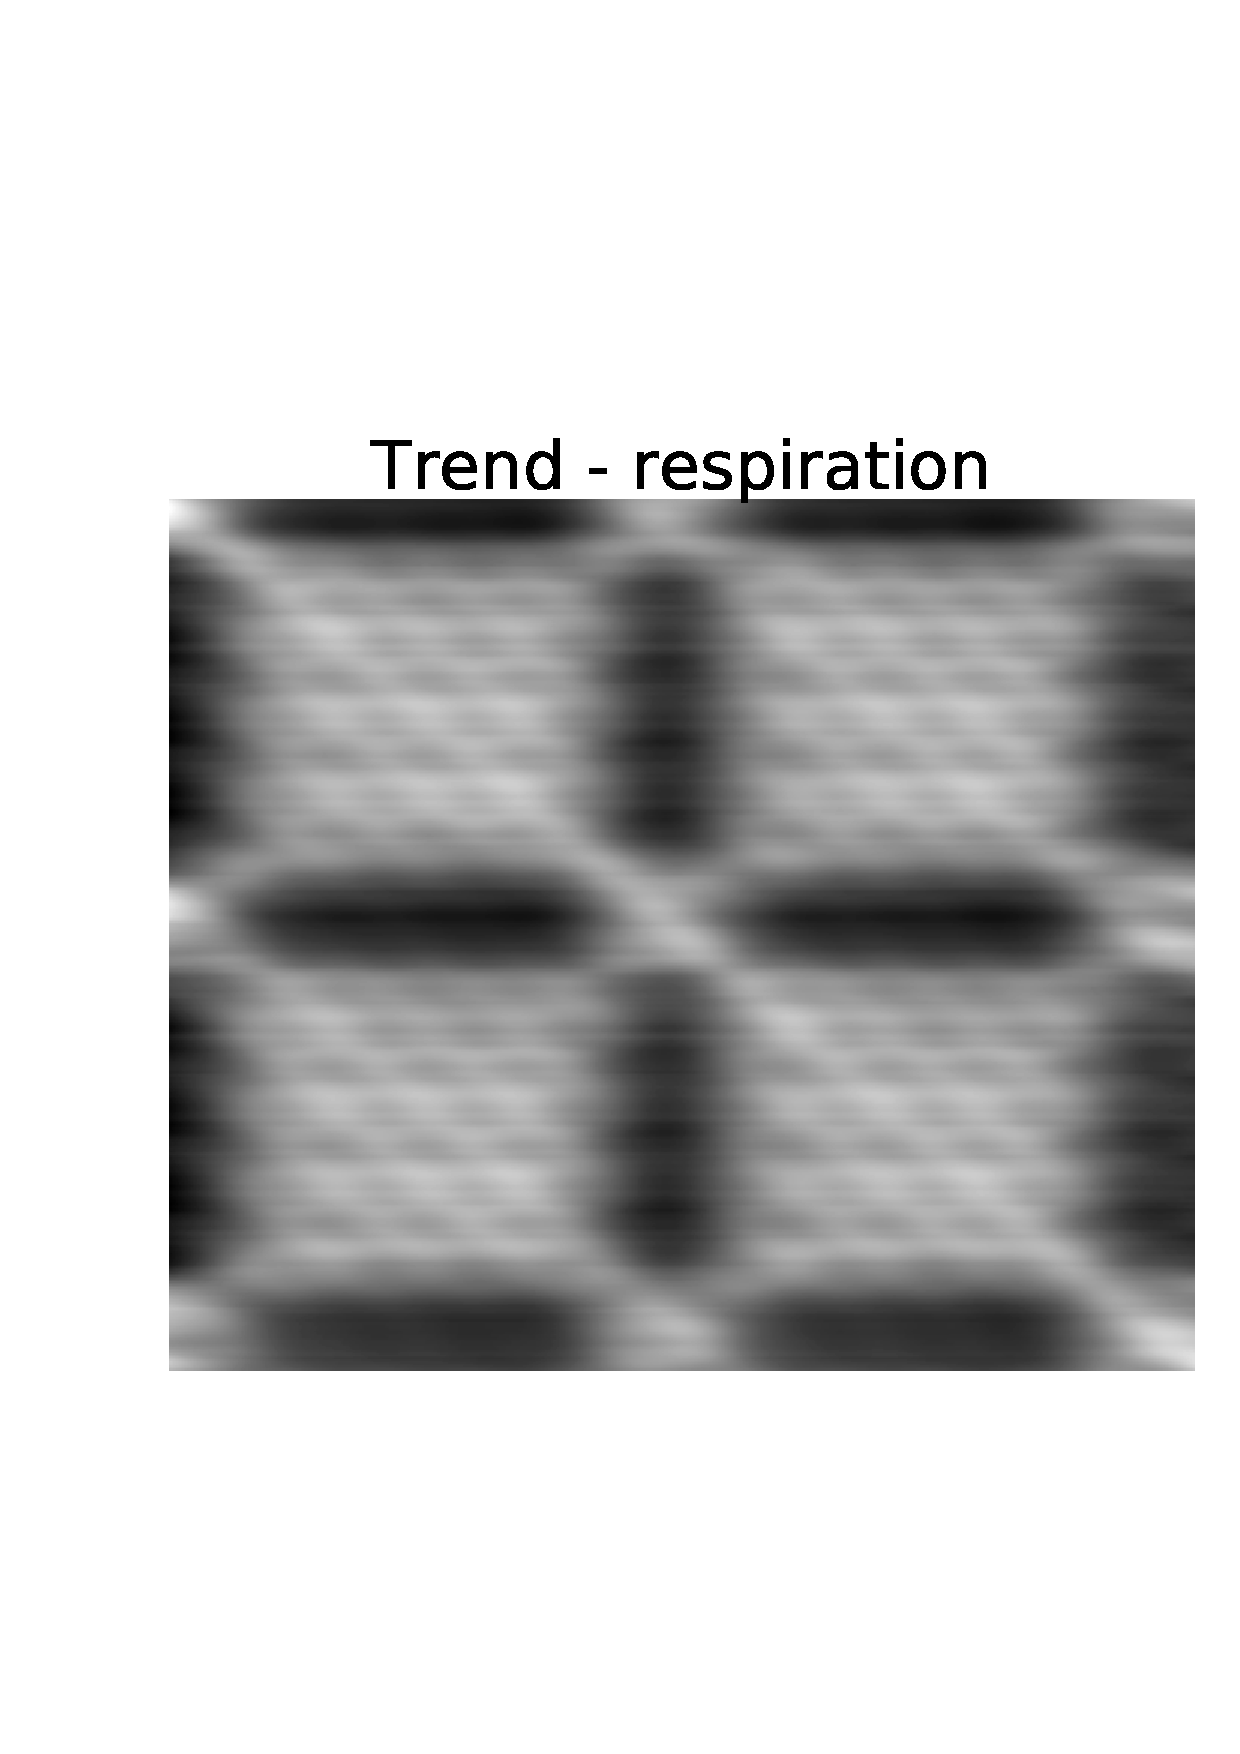
\includegraphics[width=4.75in]{figures/decoded/2015-07-27-10-36-06_2015-07-15-16-56-16_1.raw.bmode/simMat.png}
\ionbox{4.75in}\\
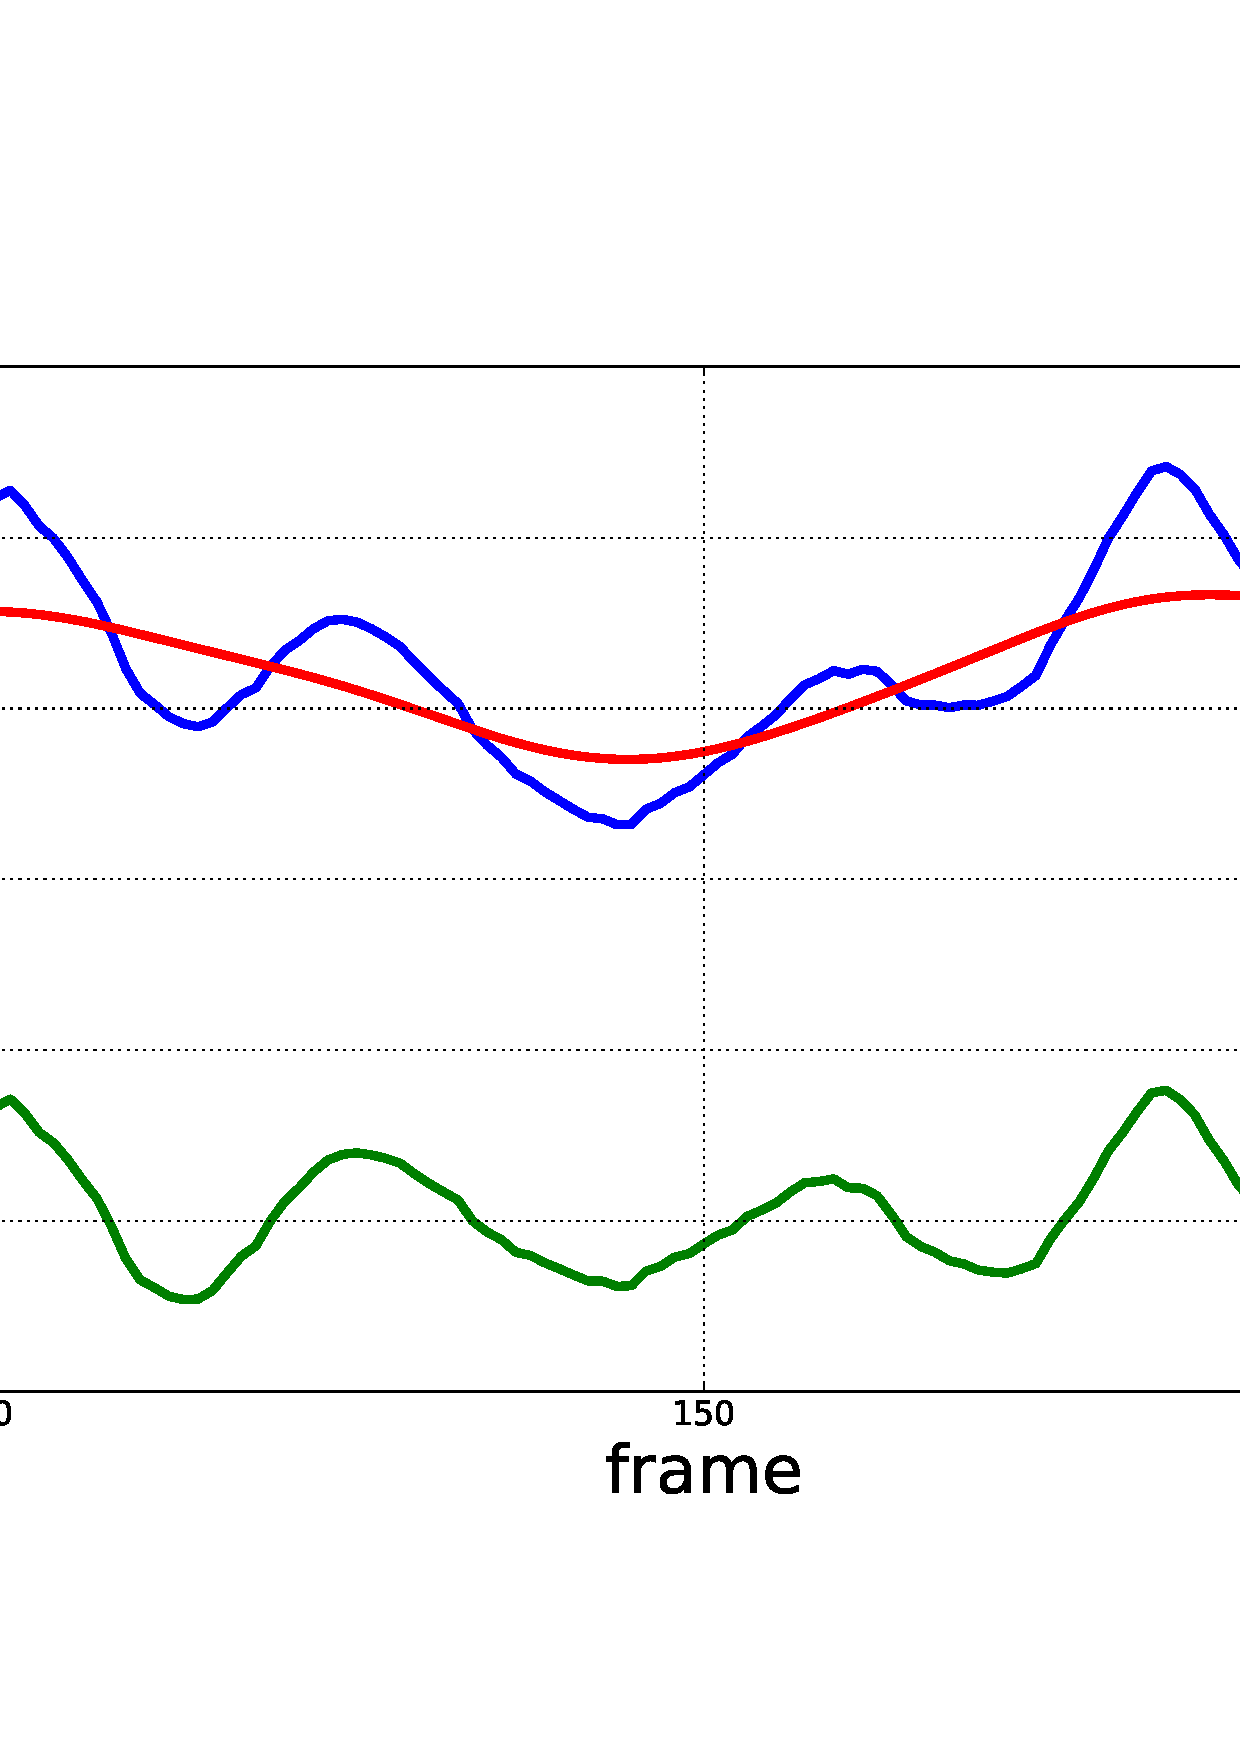
\includegraphics[width=4.75in]{figures/decoded/2015-07-27-10-36-06_2015-07-15-16-56-16_1.raw.bmode/season_trend_decomposition.png}
\ionbox{4.75in}\\
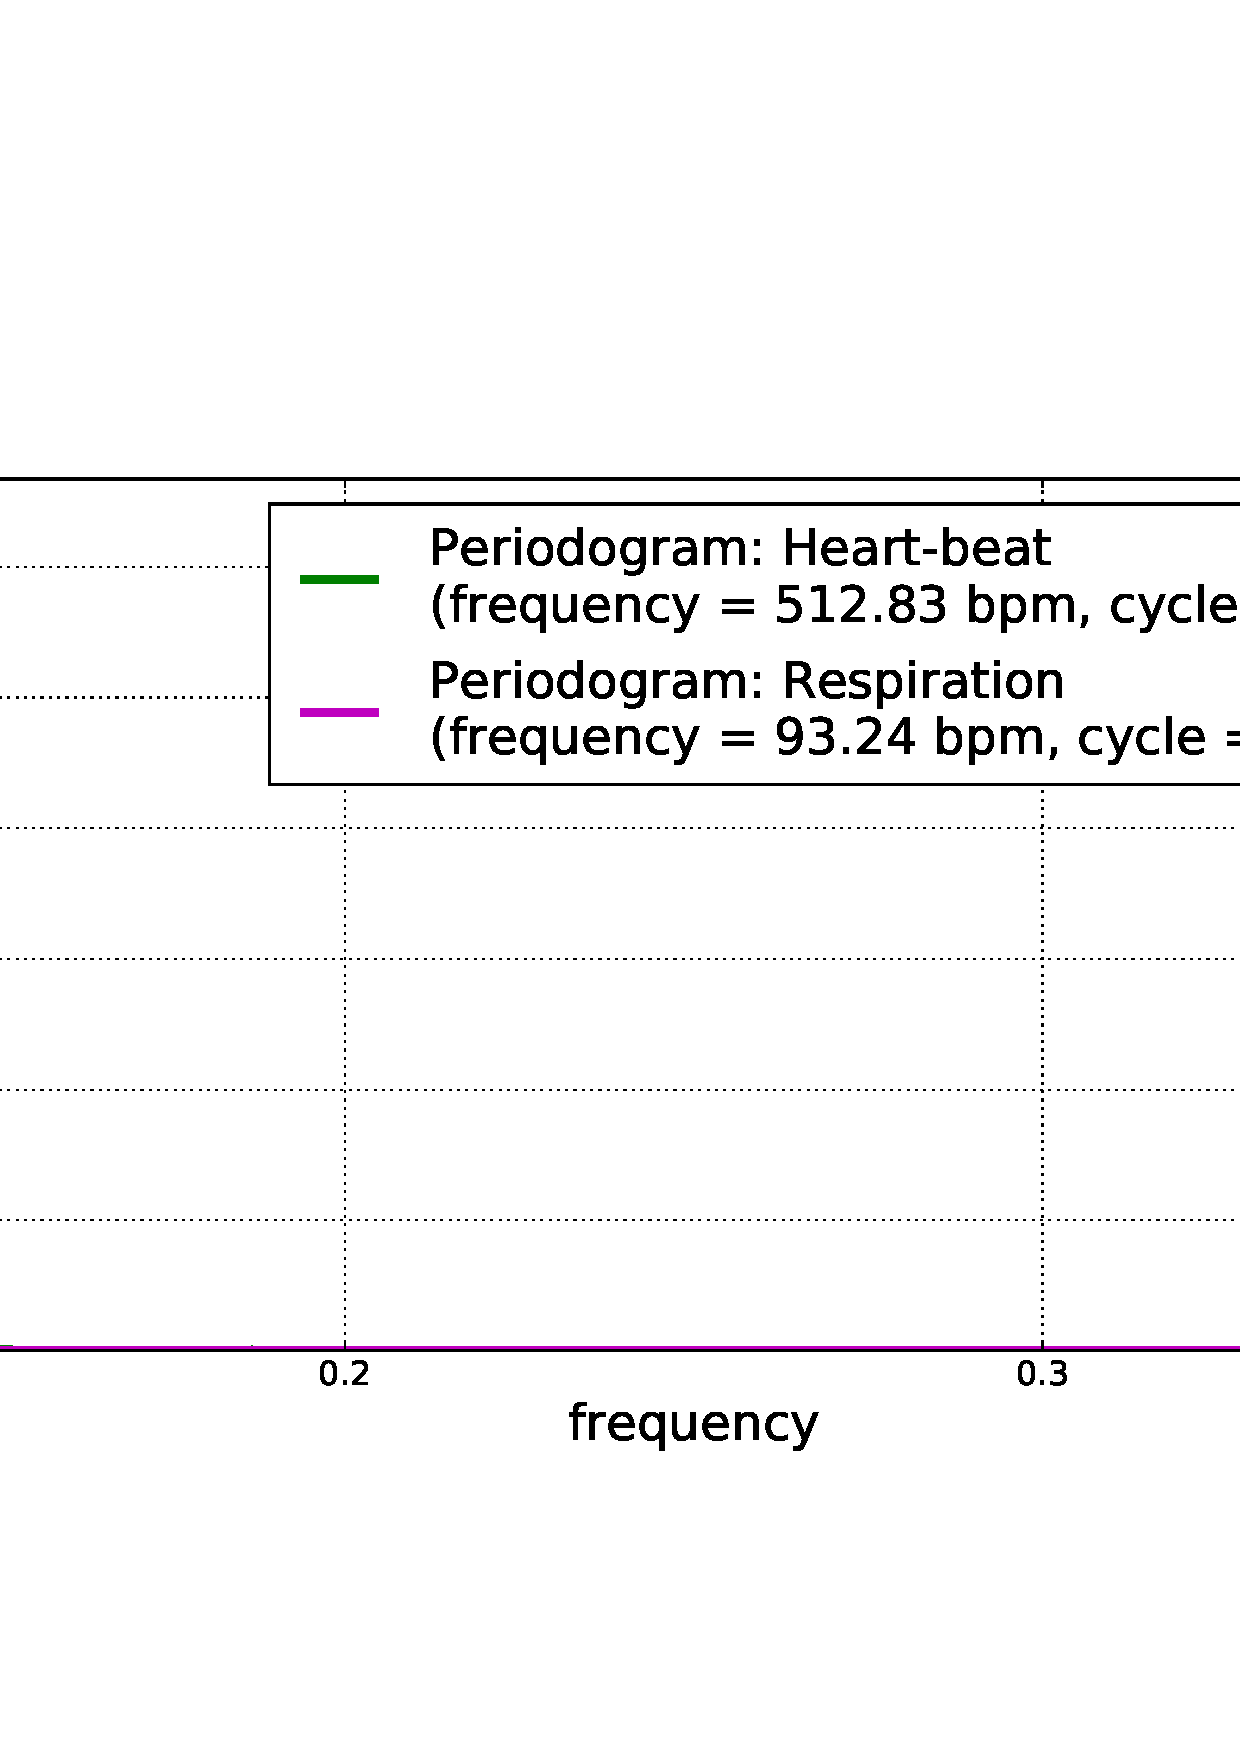
\includegraphics[width=4.75in]{figures/decoded/2015-07-27-10-36-06_2015-07-15-16-56-16_1.raw.bmode/periodogram.png}
\ionbox{4.75in}\\
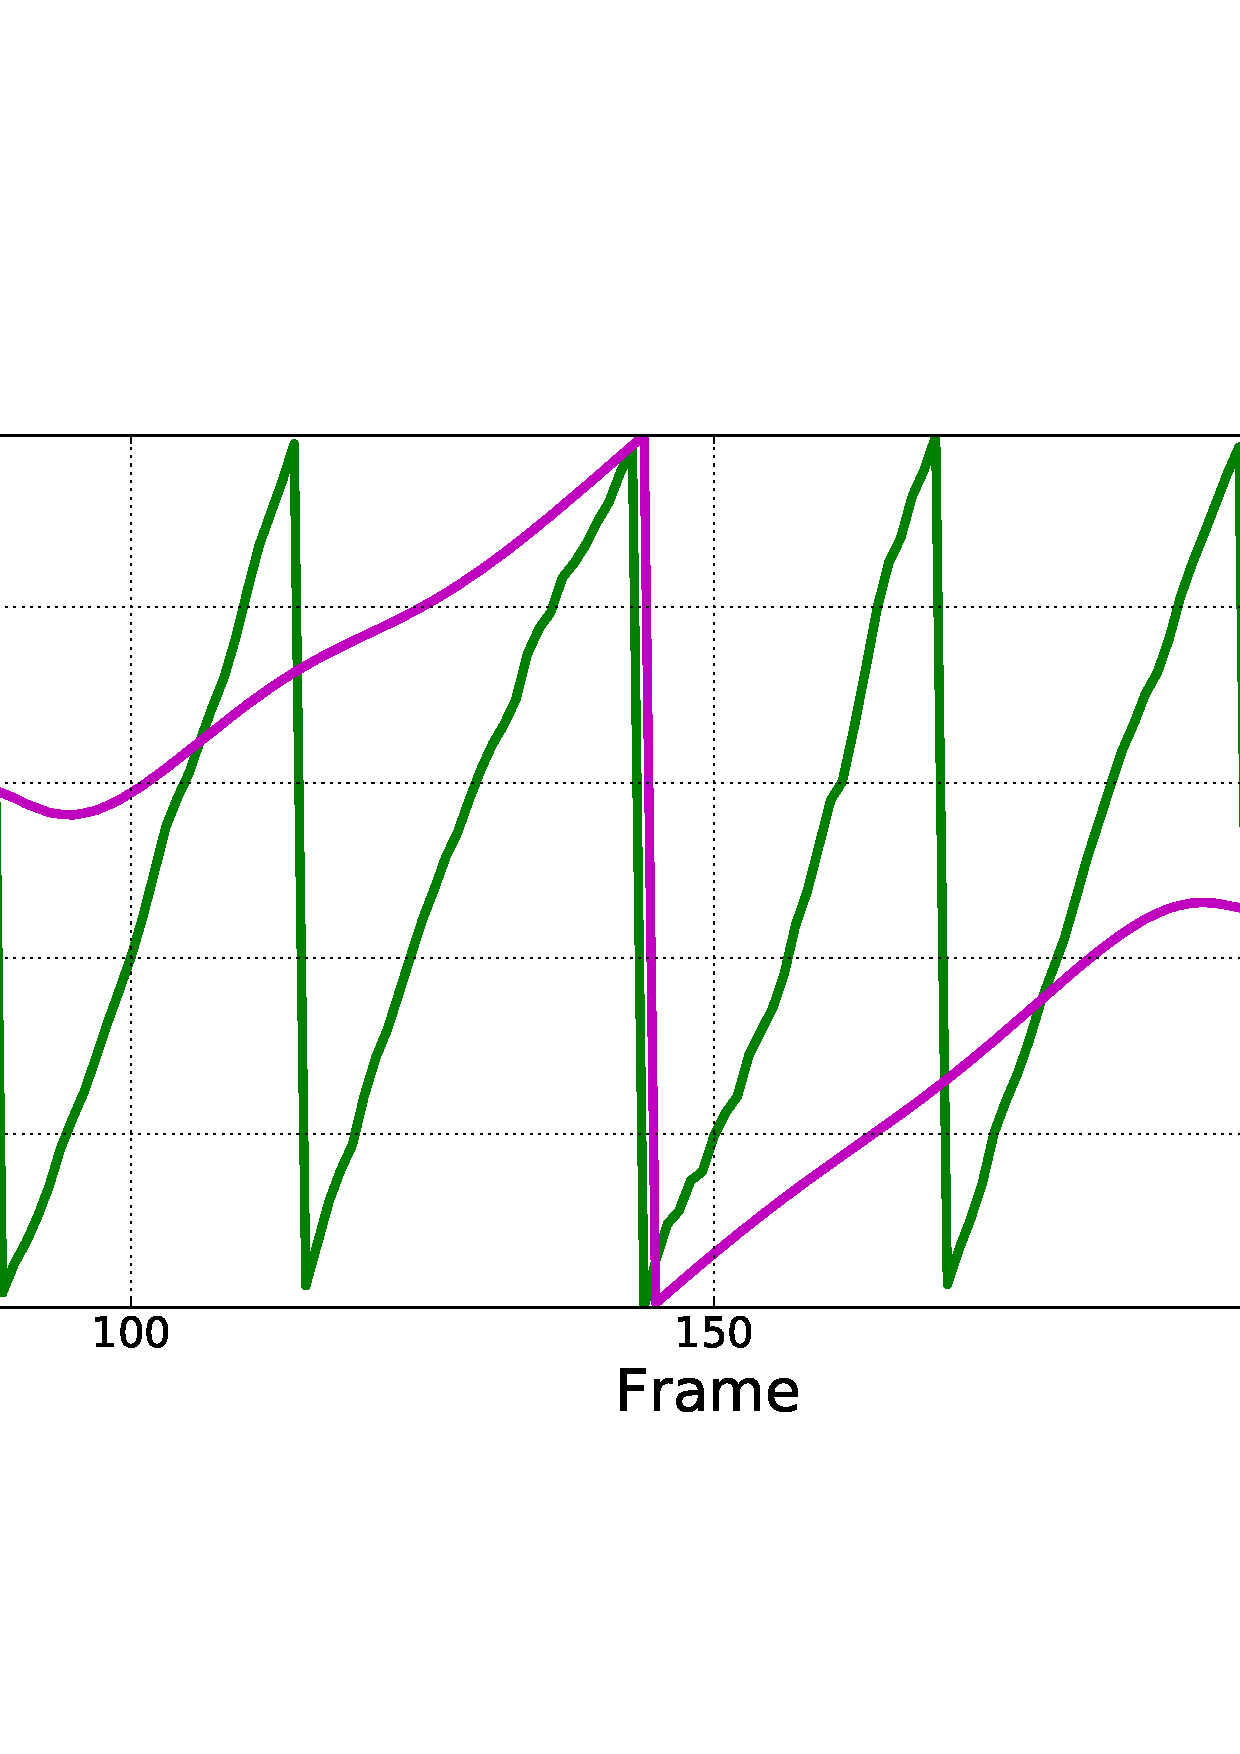
\includegraphics[width=4.75in]{figures/decoded/2015-07-27-10-36-06_2015-07-15-16-56-16_1.raw.bmode/instantaneous_phase.png}
\ionbox{4.75in}\\
%
\caption{Illustration of the proposed phase estimation method: (a-left) Inter-frame similarity matrix, (a-mid) Trend component corresponding to the respiratory motion, (a-right) Seasonal component corresponding to the beating heart motion, (b) Similarity profile with minimum spectral entropy along with the associated trend/respiration and seasonal/heart-beat components, (c) Periodogram of the heart-beat and respiration components, and (d) Instantaneous phase of heart-beat and respiration components.}
\label{fig:phase_estimation}
\end{IonFigT}
%
While there have been numerous efforts for the estimation of instantaneous phase and/or frequency in periodic univariate time series data (wherein a single-variable is measured at each time point)\cite{Boashash1992,Lu2013,Luo2003}, we are not aware of any methods that tackle this problem in a multivariate setting which is the case with cardiac ultrasound videos wherein several thousands of variables (intensities of pixels) could be measured at each time point. Our strategy was to find a way to simplify this seemingly complex multi-variate problem by transforming it into a univariate one and take advantage of existing univariate methods to solve the problem at hand. To accomplish this, we compute the similarity/affinity between all pairs of frames in the given periodic image sequence containing $n$ images to create a matrix $A \in R^{n \times n}$ where in the element $A(i,j)$ is equal to the similarity between the $i^{th}$ and $j^{th}$ frames of the given sequence. Here in, we use normalization correlation also known as the Pearson correlation coefficient to quantify inter-frame similarity but, in principle, any of the similarity metrics used in image registration algorithms \cite{Goshtasby2012} can potentially be chosen. Each row in the inter-frame similarity matrix $A$ can now be seen as a univariate time series that measures the similarity of the corresponding frame in the image sequence with all other frames. Additionally, for a periodic image sequence, we can expect them to be periodic provided that the corresponding frame is not significantly corrupted by distortions such as noise and changes in global illumination over time among others. 

To mitigate the potential problem of global illumintation changes over time, we detrend and extract the seasonal part of the time series corresponding to each row of $A$ by dividing it with the trend signal estimated using a locally-weighted regression algorithm called loess\cite{Cleveland1990}. Let $A_s$ be the matrix whose rows contain the seasonal part obtained by detrending the corresponding row in $A$. Next, we minimize the risk from noise, by finding the row $u(t)$ of $A_s$ whose power spectrum or periodogram has minimum entropy. In our experiments, the time series $u(t)$ was nearly sinusoidal in morphology with most of its energy in its power spectrum concentrated within a very narrow-band with the same periodicity characteristics as the image sequence it was derived from. Based on this observation, we decided to use its Hilbert transform \cite{Lu2013} to estimate the instantaneous intra-period phase  of each frame. Specifically, we compute the instantaneous phase $\phi(t) \in \left [  -\pi, \pi\right )$ of the time series $u(t)$ as follows:
\begin{equation}
\phi(t) = arctan \left( \frac{H_u(t)}{u(t)}\right)
\end{equation} 
where $H_u(t)$ is the Hilbert transform of $u(t)$. Lastly, we map the instantaneous phase $\phi(t)$ to the range $\left [  0, 1\right )$ which can then be used to obtain the intra-period phase of each frame.

%\vspace{-0.5cm}
\subsection{Gating out respiratory frames}
\label{sec:method:gating}
%
Once the instantaneous cardiac and respiratory phases of each frame has been estimated, it can be used to facilitate the extraction of quantitative measurements from a desired part/point of the periodic cycle, a process commonly referred to as gating. In this section, we present a robust method that uses these phase estimates to gate out video frames predominantly influenced by respiratory motion.
%
\begin{IonFigT}
\centering
%
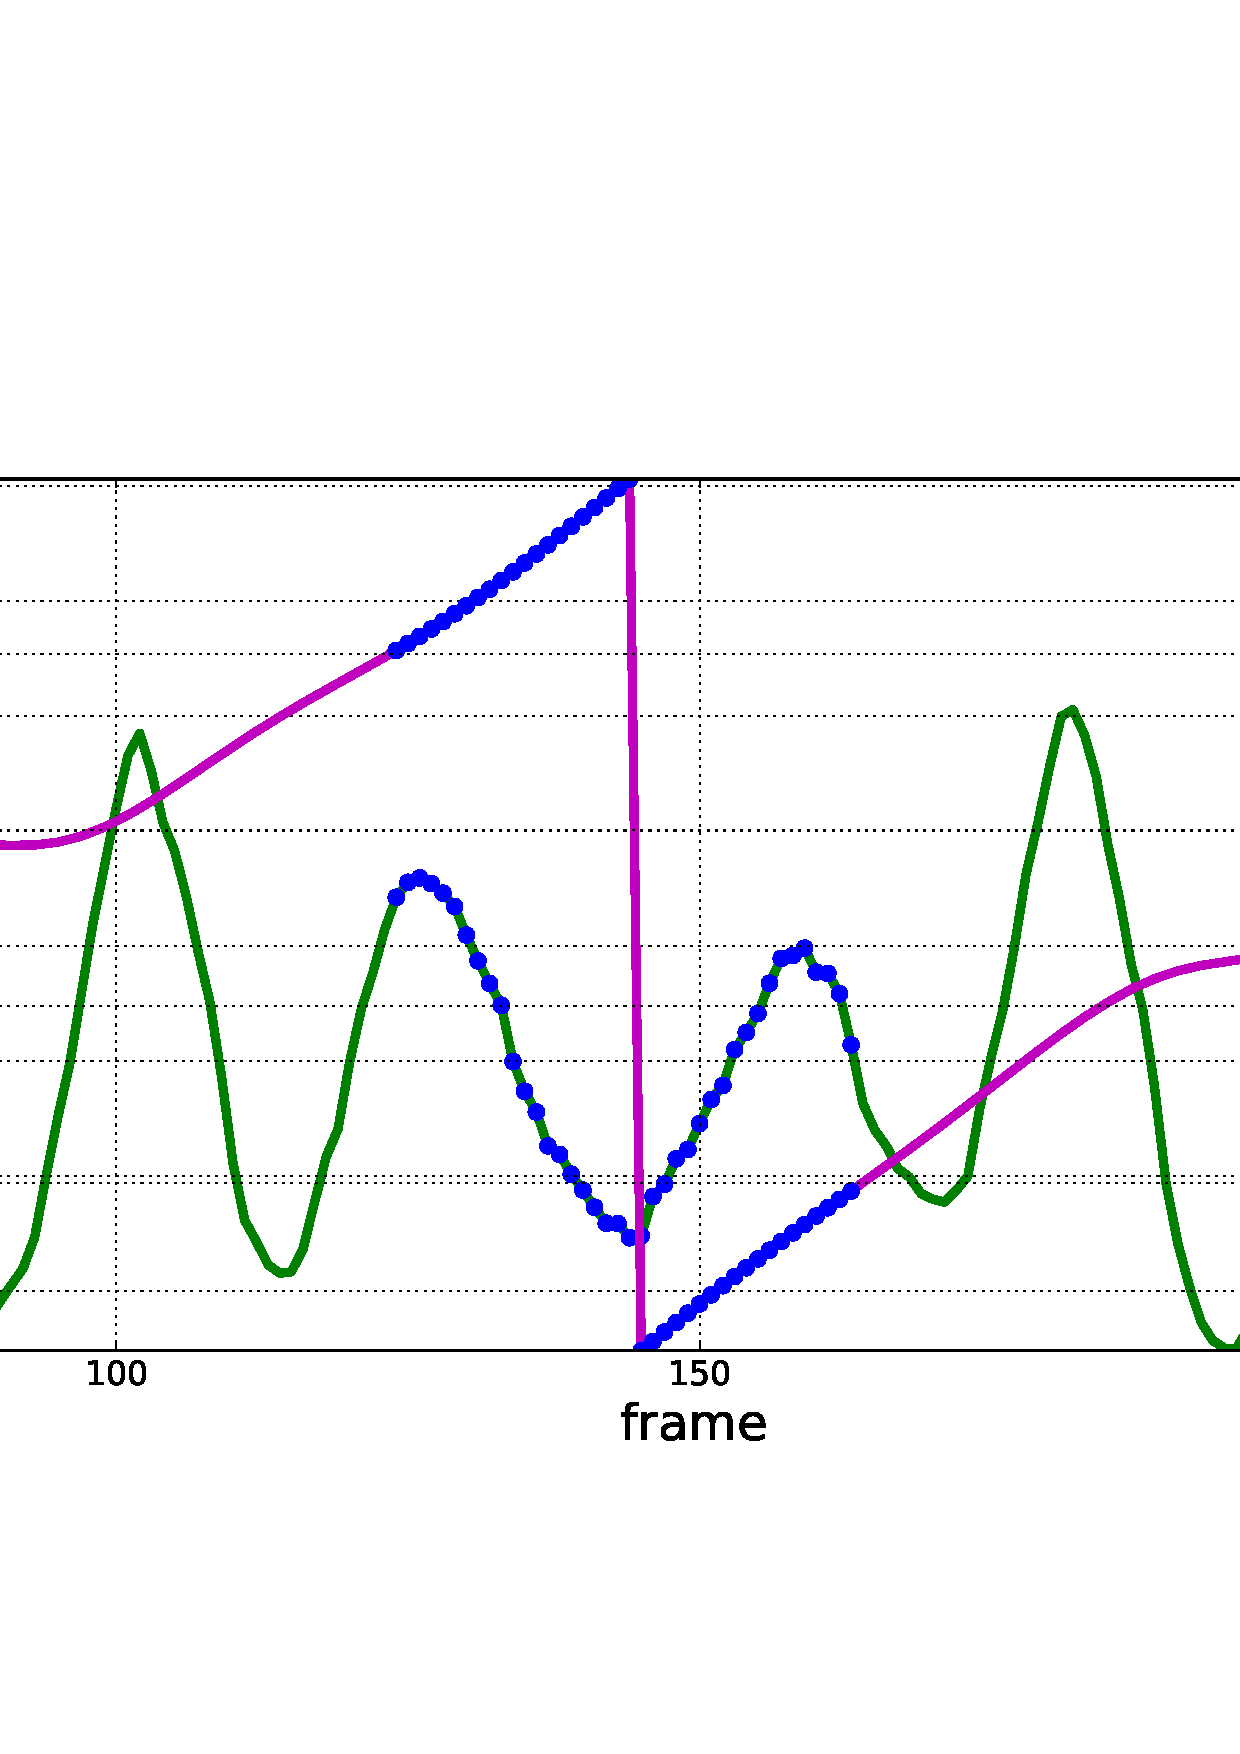
\includegraphics[width=5.0in]{figures/decoded/2015-07-27-10-36-06_2015-07-15-16-56-16_1.raw.bmode/respiratory_phase_gating.png}
\ionbox{5.0in}\\
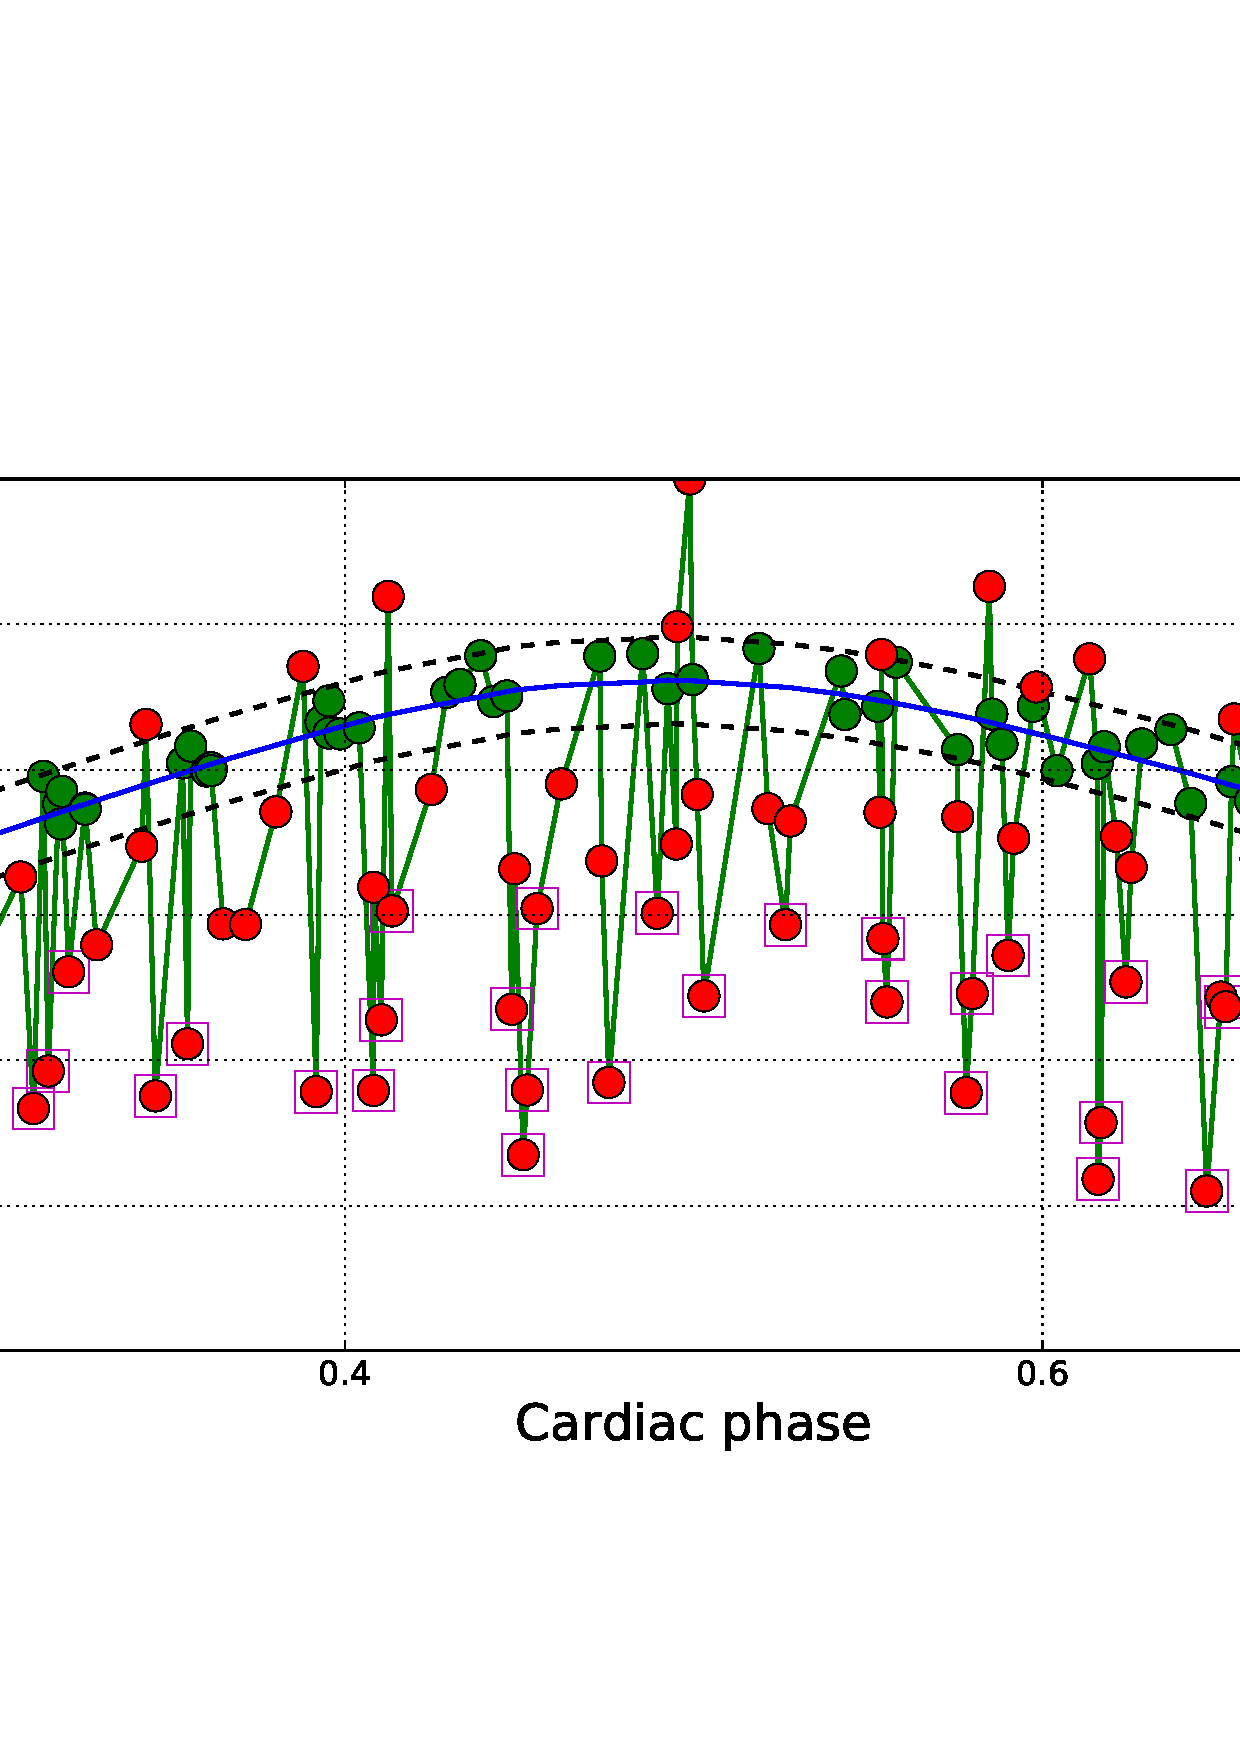
\includegraphics[width=5.0in]{figures/decoded/2015-07-27-10-36-06_2015-07-15-16-56-16_1.raw.bmode/robust_lowess_gating.png}
\ionbox{5.0in}\\
%
\caption{Illustration of our method for gating out respiratory frames: (a) (b)}
\label{fig:respiratory_gating}
\end{IonFigT}
%
%\vspace{-0.5cm}
\subsection{Reconstruction of one-period video at high temporal resolution}
\label{sec:method:super_resolution}
%
Once the instantaneous cardiac phase of each frame has been estimated, it can be used to enable spatio-temporal super-resolution by considering the set of images within each period of a periodic image sequence as distinct observations of the same data. In this section, we present a method that uses a phase-tagged periodic image sequence to reconstruct a single-period video at a higher temporal resolution. 
	
Given a de-noised periodic sequence $\{L_1, ..., L_n\}$ of $n$ images (with $m$ pixels each) along with their estimated intra-period phases $\{\phi_1, ..., \phi_n\}$, we first use Nadarya-Watson kernel regression\cite{Bishop2006} to construct a phase-parameterized image manifold in the form of a function $M(\phi): [0, 1) \to R^m $ that maps any intra-period phase $\phi$ to an image as follows:
\begin{equation}
M(\phi) = \frac{\sum_{i = 1}^{n} K(\phi, \phi_i) L_i}{\sum_{i = 1}^{n} K(\phi, \phi_i)} 
\end{equation}
where in we define the kernel $K$ using a gausssian with standard-deviation $\sigma$ equal to a multiple of the average distance between consecutive phases after sorting them. Note that, we account for the periodic nature of the intra-period phase whenever we measure distance between two phase values. A single-period video can now be reconstructed by sampling the manifold $M(\phi)$ at any desired resolution from the range $[0, 1)$ of intra-period phase. Note that the aformentioned process will facilitate temporal super-resolution only if the set of images observed in each distinct period of the given image sequence differ in intra-period phase by some non-zero amount less than its temporal sampling interval. Also, the amount of temporal super-resolution possible will depend both on the number of periods observed and the maximum amount by which one can expect the images to be perturbed in phase across observations. 
%\vspace{-0.5cm}
\section{Results}
\label{sec:results}
%
%
\begin{IonFigT}
\centering
%
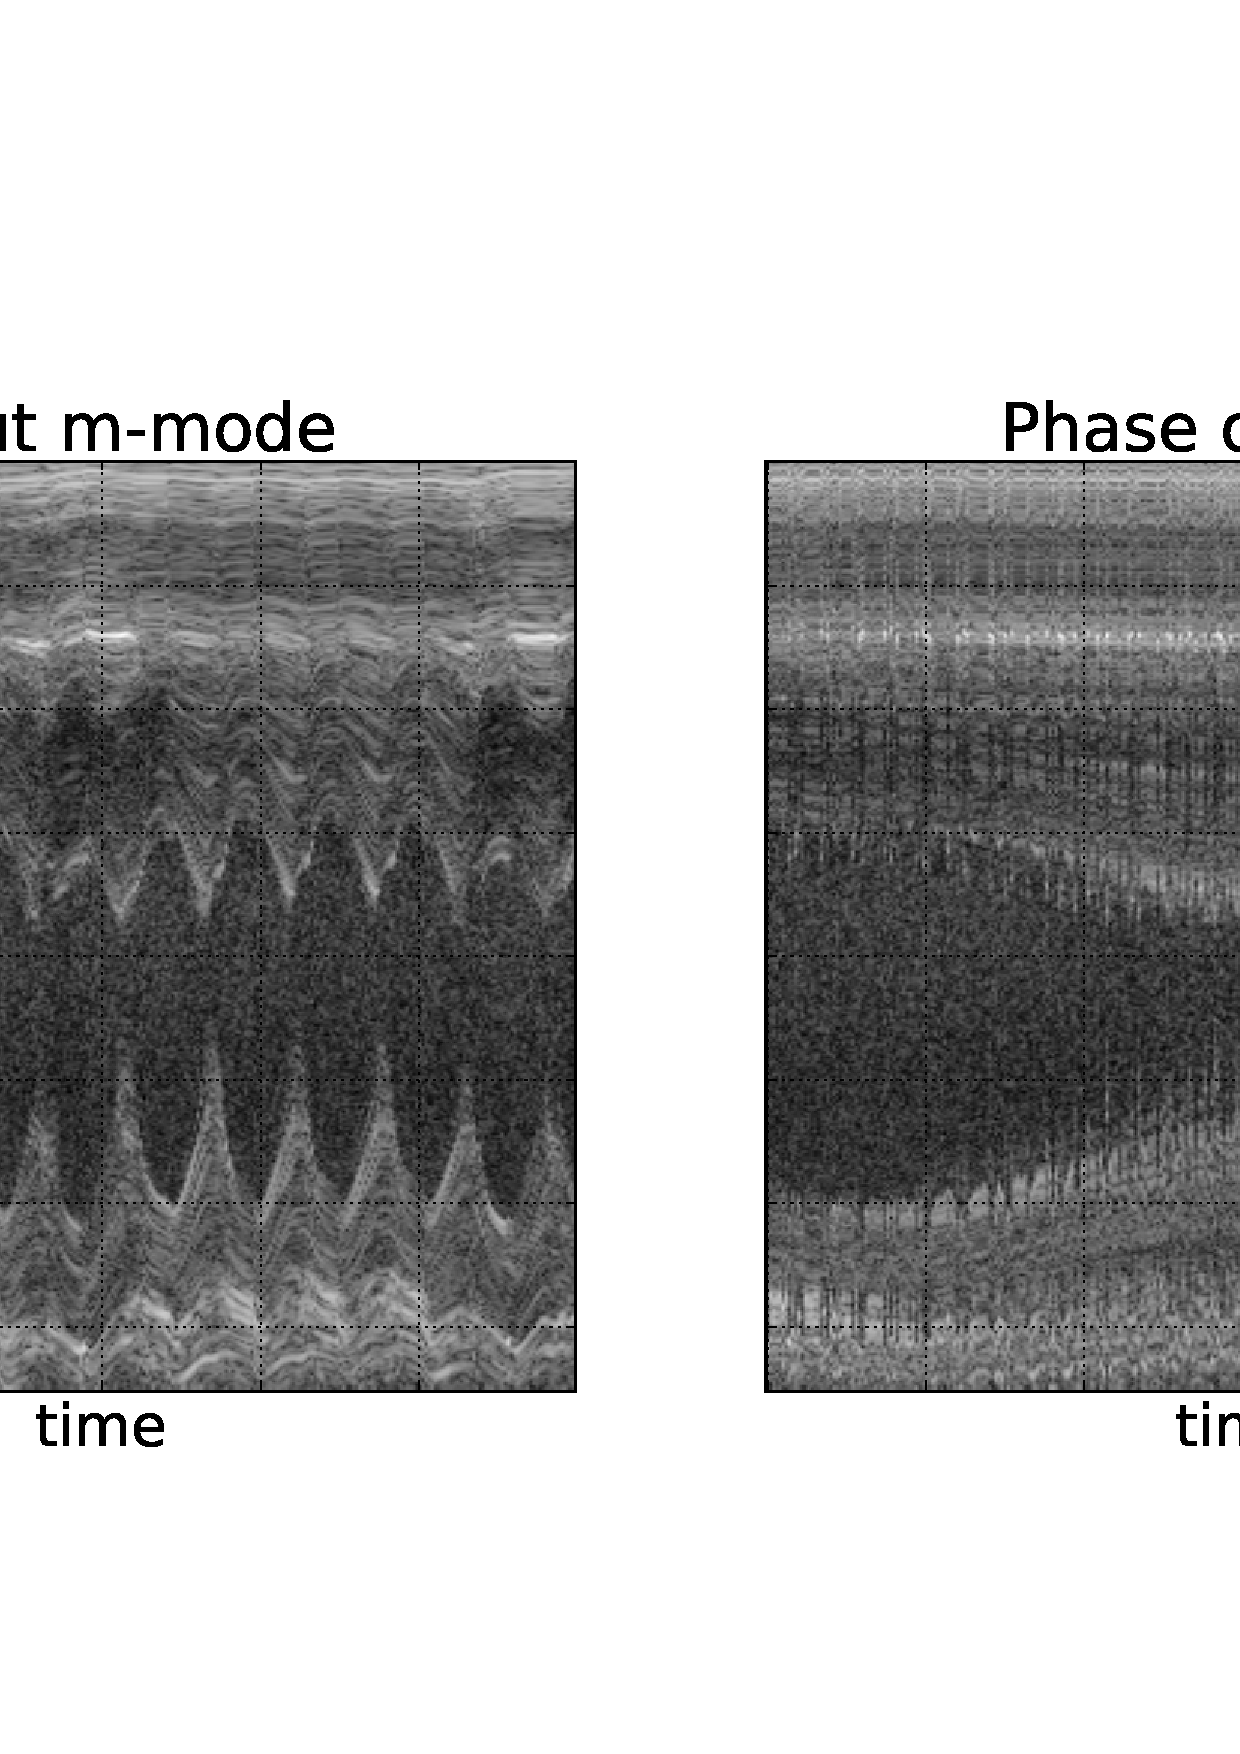
\includegraphics[width=5.0in]{figures/decoded/2015-07-27-10-36-06_2015-07-15-16-56-16_1.raw.bmode/phaseordered.png}
\ionbox{5.0in}\\
%
\caption{Visualization of m-mode frames ordered by estimated cardiac phase}
\label{fig:phase_ordering}
\end{IonFigT}
%
%
%\vspace{-0.5cm}
\section{Discussion and future work}
\label{sec:discussion}
%


%
%\vspace{-0.5cm}
\bibliographystyle{splncs03}
\bibliography{library}
\end{document}







